\section{Zometool construction}
\label{sec:Zometool}

\begin{figure}[ht]
\centering
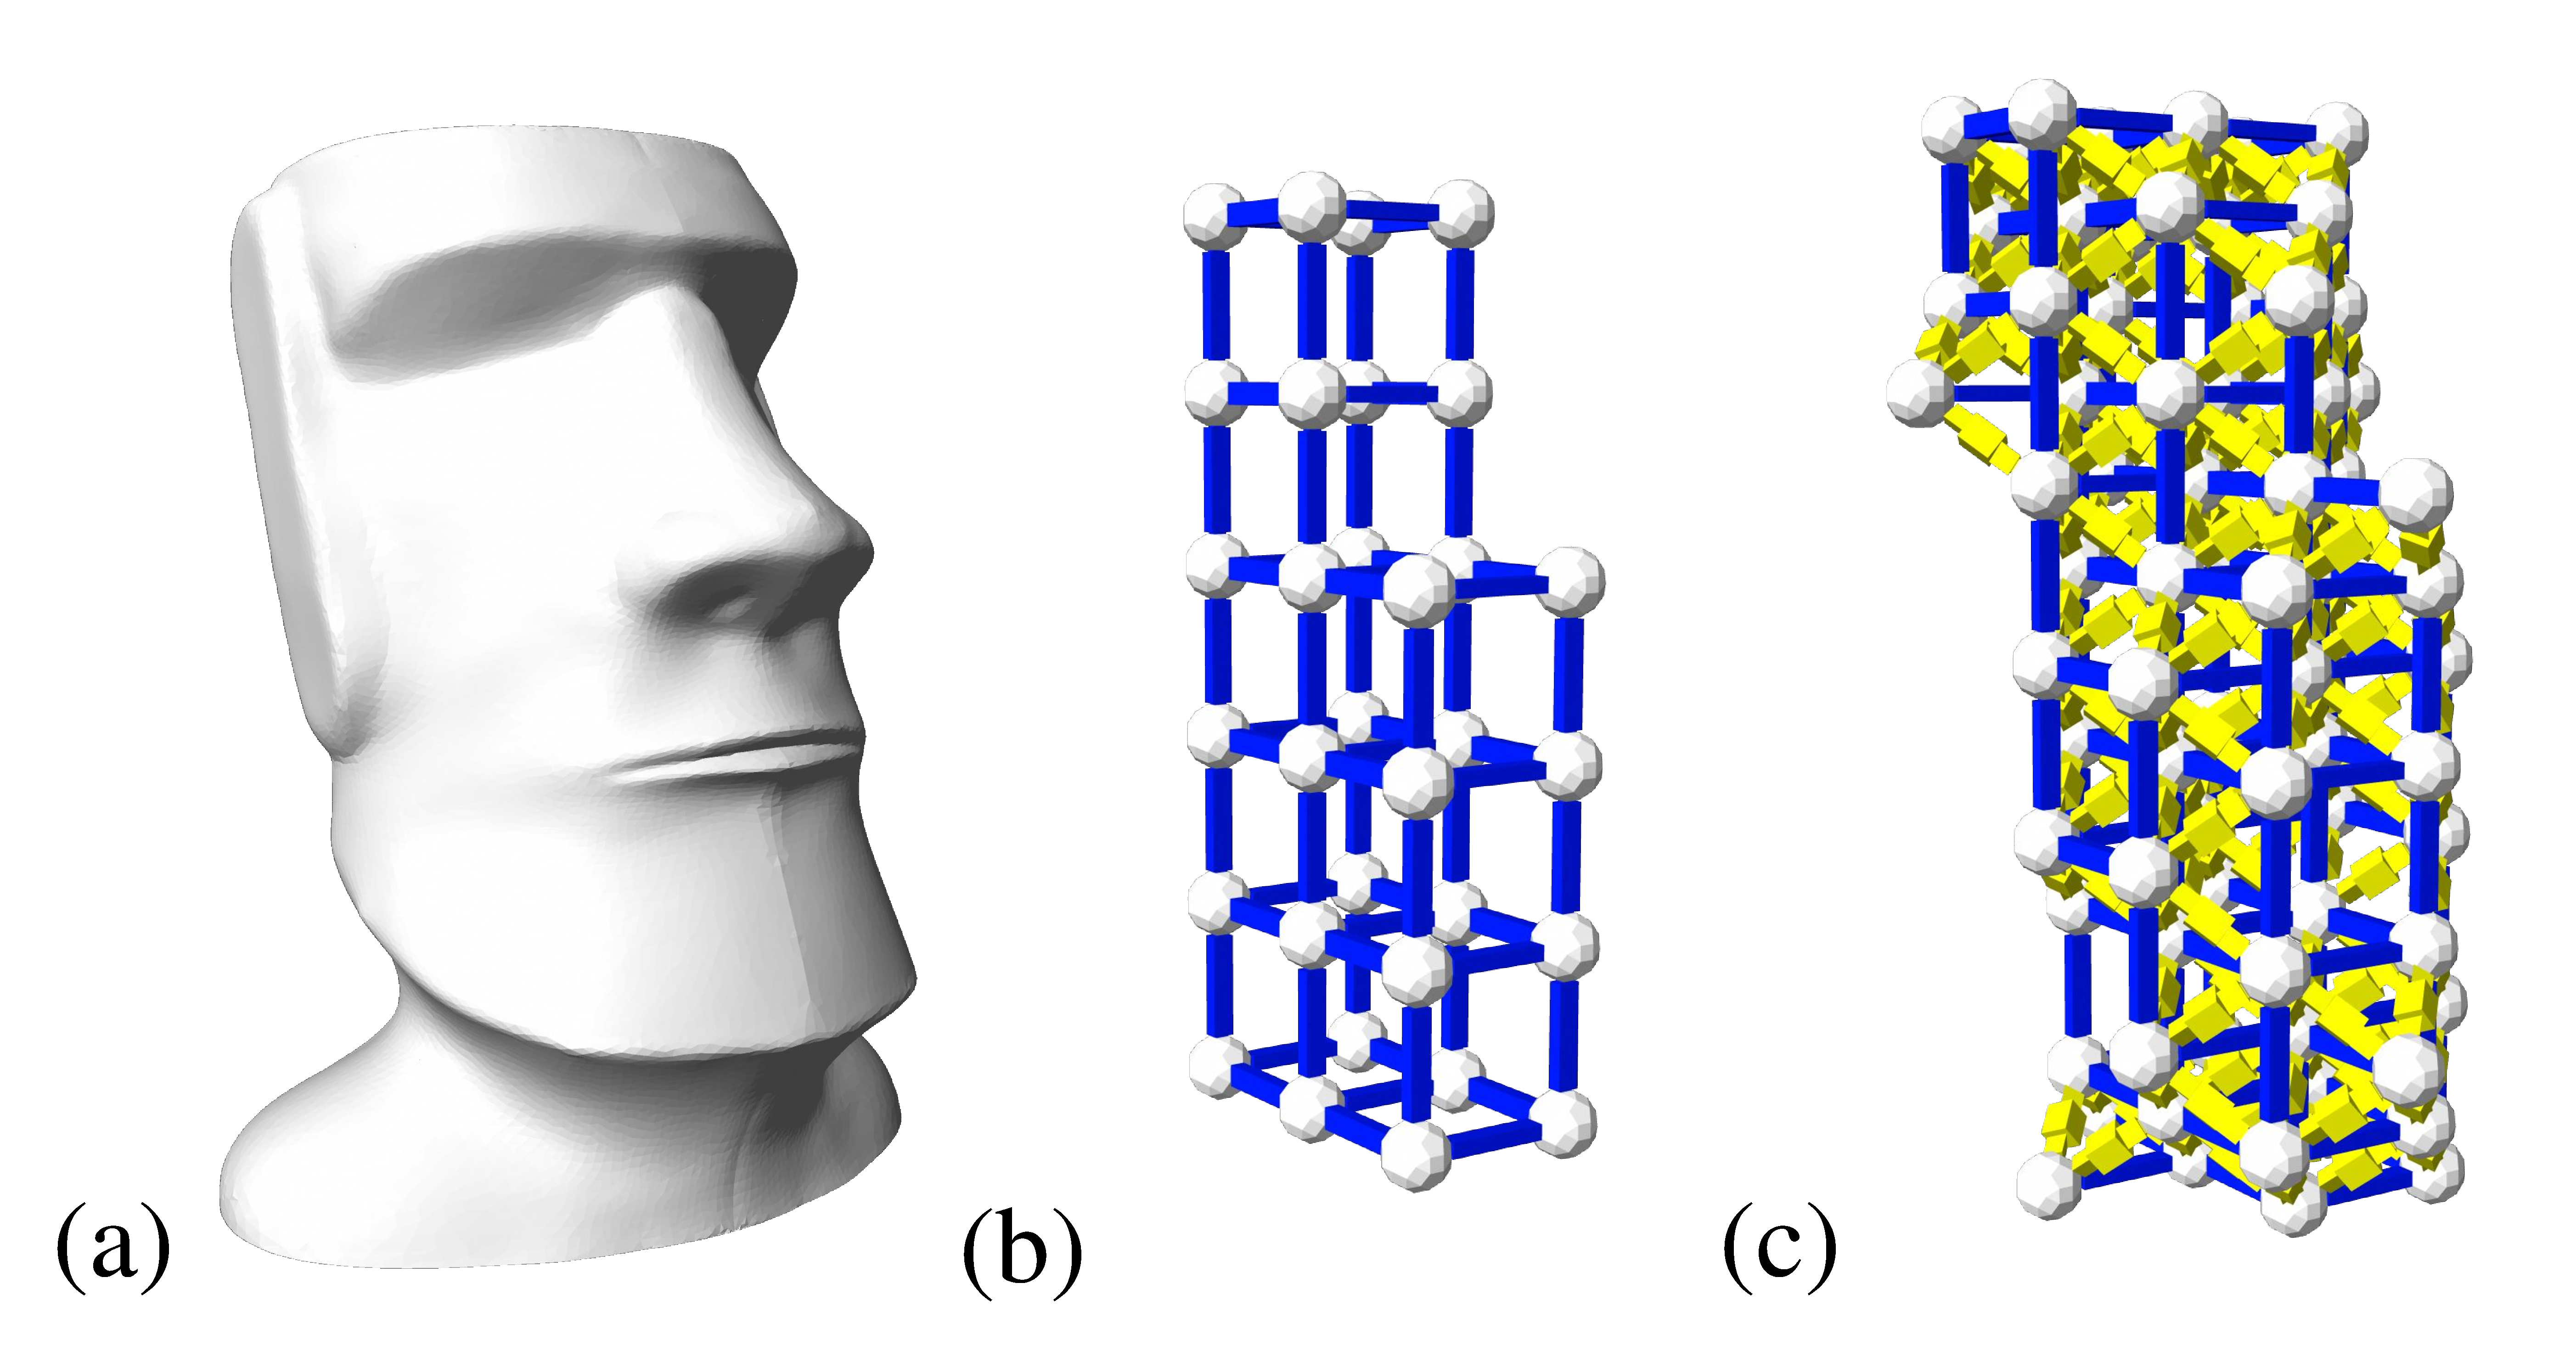
\includegraphics[width=\linewidth]{figs/Zometool_init.pdf} 
\caption{
\ichao{this figure is too space wasting..Maybe just put a small cube as inset in the corresponding location in paper.}
Given input shape (a), we initialize the Zometool structure with cubes (b), and obtain the optimized result (c) by using Simulated Annealing as described in \secname~\ref{sec:Zometool}.}
\label{fig:Zometool_cont}
\end{figure}

% The goal of our method is devising an algorithm to construct an object composed of Zometool structures and 3D-printed parts with the following objectives:
% \begin{itemize}
%     \item \textit{material-effecitiveness} We should aim to minimize the overall fabrication cost and time.
%     Since Zometool is substantially faster to build and reusable, we should maximize it's usage to reduce 3D printing material in the fabrication.
%     \item \textit{easy-to-assemble} We should reduce the difficulties of assemble both Zometool structure and outer printed shell. In terms of Zometool, we should minimize the usage of nodes and rods, so to reduce the assemble time.
% \end{itemize}

\subsection{Introduction to Zometool}
Zometool is widely used as educational toys to replicate complicated scientific structures such as chemical structures. 
The rods in standard Zometool system have three different types tenons, \ie~blue for rectangle, red for pentagonal and yellow for triangle.
Each type of rod also has three different sizes (see \figname~\ref{fig:Zometool}).
We denote $(b_0$, $b_1$, $b_2)$ as three different lengths of blue rods ($(r_0$, $r_1$, $r_2)$ for red rod, and $(y_0$, $y_1$, $y_2)$ for yellow rod).
% Also, $r_0$, $r_1$, $r_2$ are the red rods, and $y_0$, $y_1$, $y_2$ are for yellow rods. 
There are totally 62 slots on the Zome-ball, including 30 rectangular slots, 12 pentagonal slots and 20 triangular slots. 
% On the other hand, Zometool has a math model which we will introduce it's detail in following context.
%The Zome-ball have 62 slots on it. There are 30 rectanglular slots, 12 pentagonal slots and 20 triangular slots. Zometool have a math model in it. We will introduce it's detail in following context.
% \subsubsection{Strut lengths}
Each color of Zometool rods has three sizes, and the growing ratio is related to the golden ratio $\gamma = \frac{1+\sqrt{5}}{2}$. 
Take blue rods for example, $b_1 = b_0 \cdot \gamma$ and $b_2 = b_0 + b_1$. 
Red and yellow rods also follow this rule. 
Moreover, the relative length ratios are different from yellow to blue and red to blue, \ie~ $y_i = \frac{\sqrt{3}}{2} \cdot b_i$ and $r_i = \frac{\sqrt{2 + \gamma}}{2} \cdot b_i$.
Please refer to~\cite{davis2007mathematics} for more detail about the underlying mathematical model of Zometool.
% Moreover, the rods with different colors have their own related ratio, i.e. $y_i = \frac{\sqrt{3}}{2} \cdot b_i$ and $r_i = \frac{\sqrt{2 + \gamma}}{2} \cdot b_i$.

% \subsubsection{Zometool vectors}
% Now we know Zome-ball have 62 slots on it, and there are three different types of rods. 
% Each type of them has three different sizes. 
% If we put the Zome-ball in x-y-z coordinate, we can get 62 fix vectors which correspond to slots. And we also can get 186 positions which is from the center of Zome-ball to the end point of rods. This information can improve the accuracy in computation.

\begin{figure}[ht]
\centering
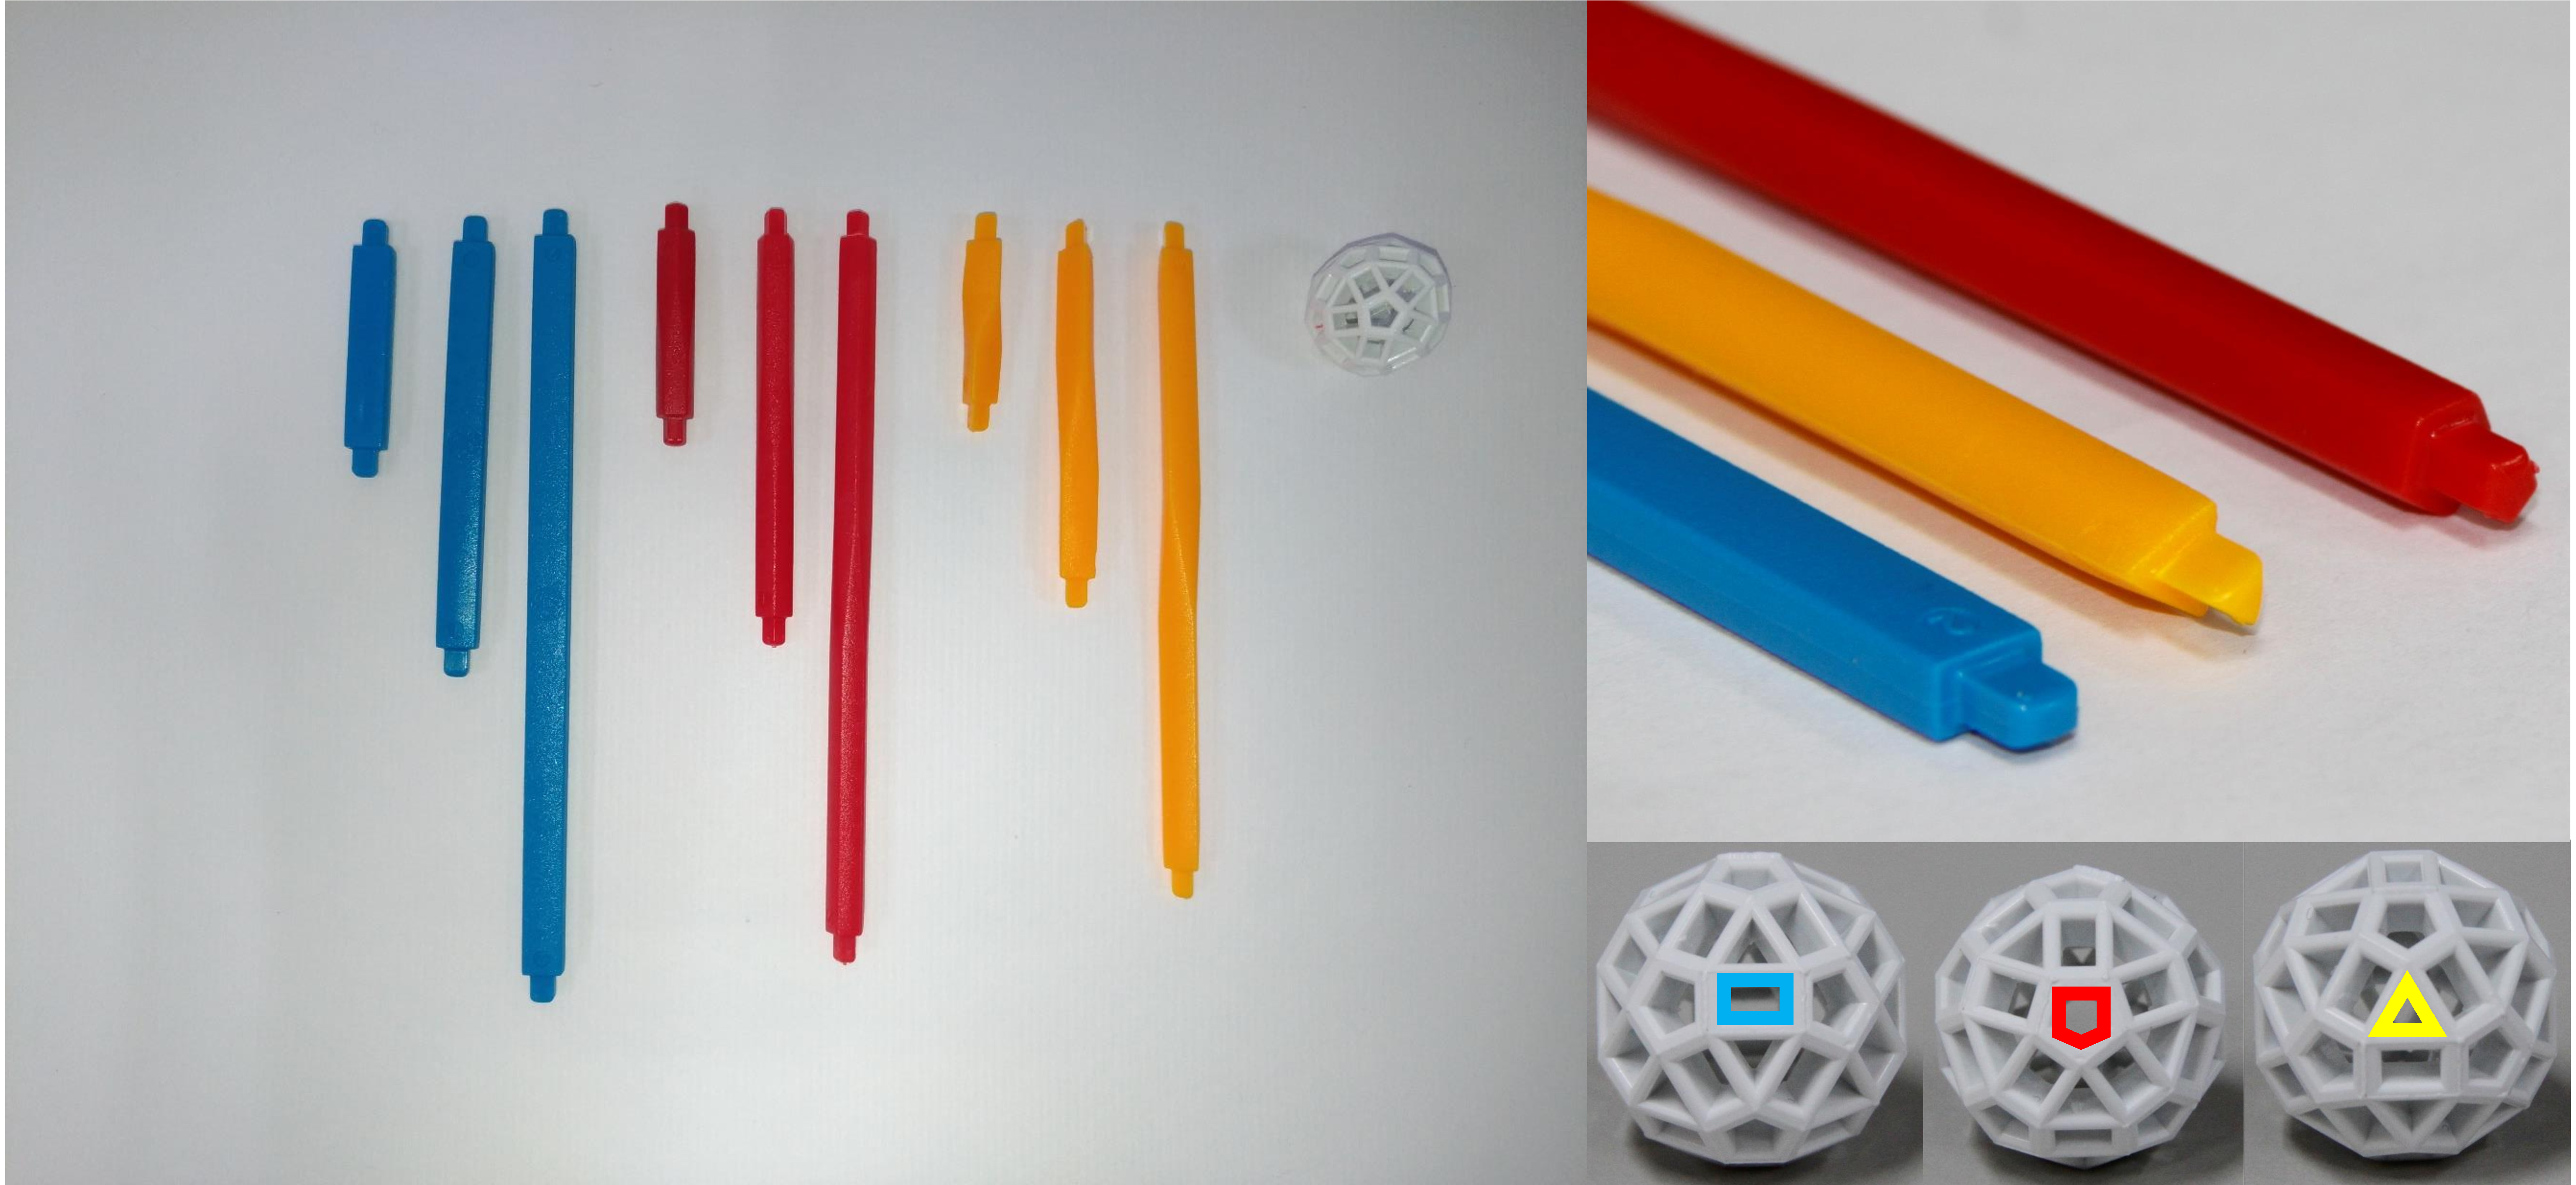
\includegraphics[width=1.0\linewidth]{figs/Zometool.pdf} 
\caption{
The standard Zometool components}
\label{fig:Zometool}
\end{figure}

\subsection{Initialization}
%We first partition $S$ into $m$ segments ($S=\{s_1, \cdots , s_m\}$) using Shape Diameter Function (SDF)~\cite{shapira:2008:consistent} and clustering implemented in CGAL~\cite{cgal}.
%First we want to fill the inner volume of each segment $s_i$.
%Although we can use some existing works~\cite{zimmer:2014:Zometool} to generate the inner Zometool structure, we intend to use structure that is composed of simple primitives because it's simplicity and easy-assembility.
%Follow Zimmer \cite{zimmer:2014:Zometool}, we choose to use cube as the basic primitive to initialize the filling.
%The initialized Zometool structure is denoted as 
%$\bar{\mathcal{Z}}=\{\mathcal{Z}_0,...,\mathcal{Z}_n\}$, 
%where $n$ is the number of segments with embedded Zome tools 
% We know the math model of Zometool and how it works in previous section, and decide the inner structure growing method. 
% The main feature of Zometool is let it can build thousands of structures. However, more complicated structure will take the more assembling time. 
Although we can assemble many complicated structures using Zometool, the assemble complexities and time consumption grows pretty fast as the number of Zometool items (rod and ball) used.
Our idea is that choosing the simple and repeated unit structure to make up the initial structure, and then growing out from main structure to get better fitting of outer surface. 
After experimenting different basic structure, such as cube, triangular pyramid, square-based pyramid and pentagonal pyramid, we choose cube as unit building block due to it's smallest assemble time.
% We find that triangular pyramid can get the best fitting but cube can get the less assembling time. 
% Finally, wants to approach our goal \textbf{fast assembling}. 
We follow Zimmer~\cite{zimmer:2014:Zometool} with cube as the basic unit to initialize the filling. 
The major difference from Zimmer~\cite{zimmer:2014:Zometool} is that we choose $b_0$ (the length of shortest blue rod) for our edge length of cube. 
The reason is that the smaller the cube is, the higher fitting rate we can achieve, and the inner structure will get closer to outer surface.
(see \figname~\ref{fig:Zometool_cont}(b) for sample initialization). 

%\section{Simulated annealing}
%After get the initial structure, the structure still too rough and weak for the inner structure. We want to more close to the outer structure and get more robust structure. But the main problem is thousand of possibility of Zometool. So we choose simulated annealing to make the problem be solved. The core of simulated annealing is design the (i) local operation, (ii) energy function and (iii) cooling schedule. The following context will discuss our design detail.


% \begin{wrapfigure}{r}{0.25\columnwidth} %this figure will be at the right
% 	\hspace{-5pt}
%   \begin{center}
%     \includegraphics[width=0.23\columnwidth]{figs/accuracyConstraints/accuracyConstraints.pdf}
%     \end{center}
%     \vspace{-5pt}
% \end{wrapfigure}

\subsection{Problem Formulation}
We measure the quality of the Zometool structure $\mathbf{Z}$ \ignore{model }with an energy $E$ which is composed of 4 terms according to different quality measurements:
\begin{align}
\label{eq:sa_energy}
E(\mathbf{Z})&=w_{\text{dist}}\cdot E_{\text{dist}}(\mathbf{Z}) + w_{\text{reg}} \cdot E_{\text{reg}}(\mathbf{Z}) \nonumber \\ 
&+ w_{\text{val}}\cdot E_{\text{val}}(\mathbf{Z}) + 
w_{\text{sim}} \cdot E_{\text{sim}}(\mathbf{Z}),
\end{align}
(we set $w_{{dist}}$ = 1.0, $w_{{reg}}$ = 100.0, $w_{{val}}$ = 1.0, $w_{{sim}}$ = 1.0 through all examples shown in this paper.)

\subsubsection{Distance}
The distance from $\mathbf{Z}$ to $S$ is integrated over all the nodes :
\begin{align}
E_{\text{dist}}(\mathbf{Z}) = \frac{1}{P\cdot d^2_{\text{norm}}} \sum_{i=1}^{P} \|p_i - \pi(p_i) \|^2 \cdot (1+F(p_i)),
\end{align}
where $P$ is the number of nodes and the normalization factor $d_{\text{norm}}$ is used to relate distance to the fixed length of the struts.
We follow \cite{zimmer:2014:Zometool} and define the term $F(p)$ called forbidden zone, which penalizes node points lying too far away from surface. 
%Please see ~\ref{forbidden} for more details.

\paragraph{Forbidden Zone}
\note{Even if long distance from surface will cause the higher energy, we still want to accelerate the process.} 
During energy computation, the distance have to multiply the additional weight which is called Forbidden zones in \cite{zimmer:2014:Zometool}. 
$F(p)$ is defined as a quadratically increasing function which depends on the distance between the triangle centroid position $p$ to the nearest node $S$. $F(p)$ will be zero when the distance is smaller than $d_{\text{min}}$ and will be $F_{\text{max}}$ when the distance is larger than $d_{\text{max}}$. 
After a series of tests, finally we get the best parameters. 
We set $d_{\text{min}}$ = 16.0 ($\frac{1}{3}$ length of $b_0$) , $d_{\text{max}}$ = 47.3 (length of $b_0$) and $F_{\text{max}}$ = 70.0 for all the examples in this paper. 
%(see \figname~\ref{fig:forbidden})\label{forbidden}

% \begin{figure}[ht]
% \centering
% 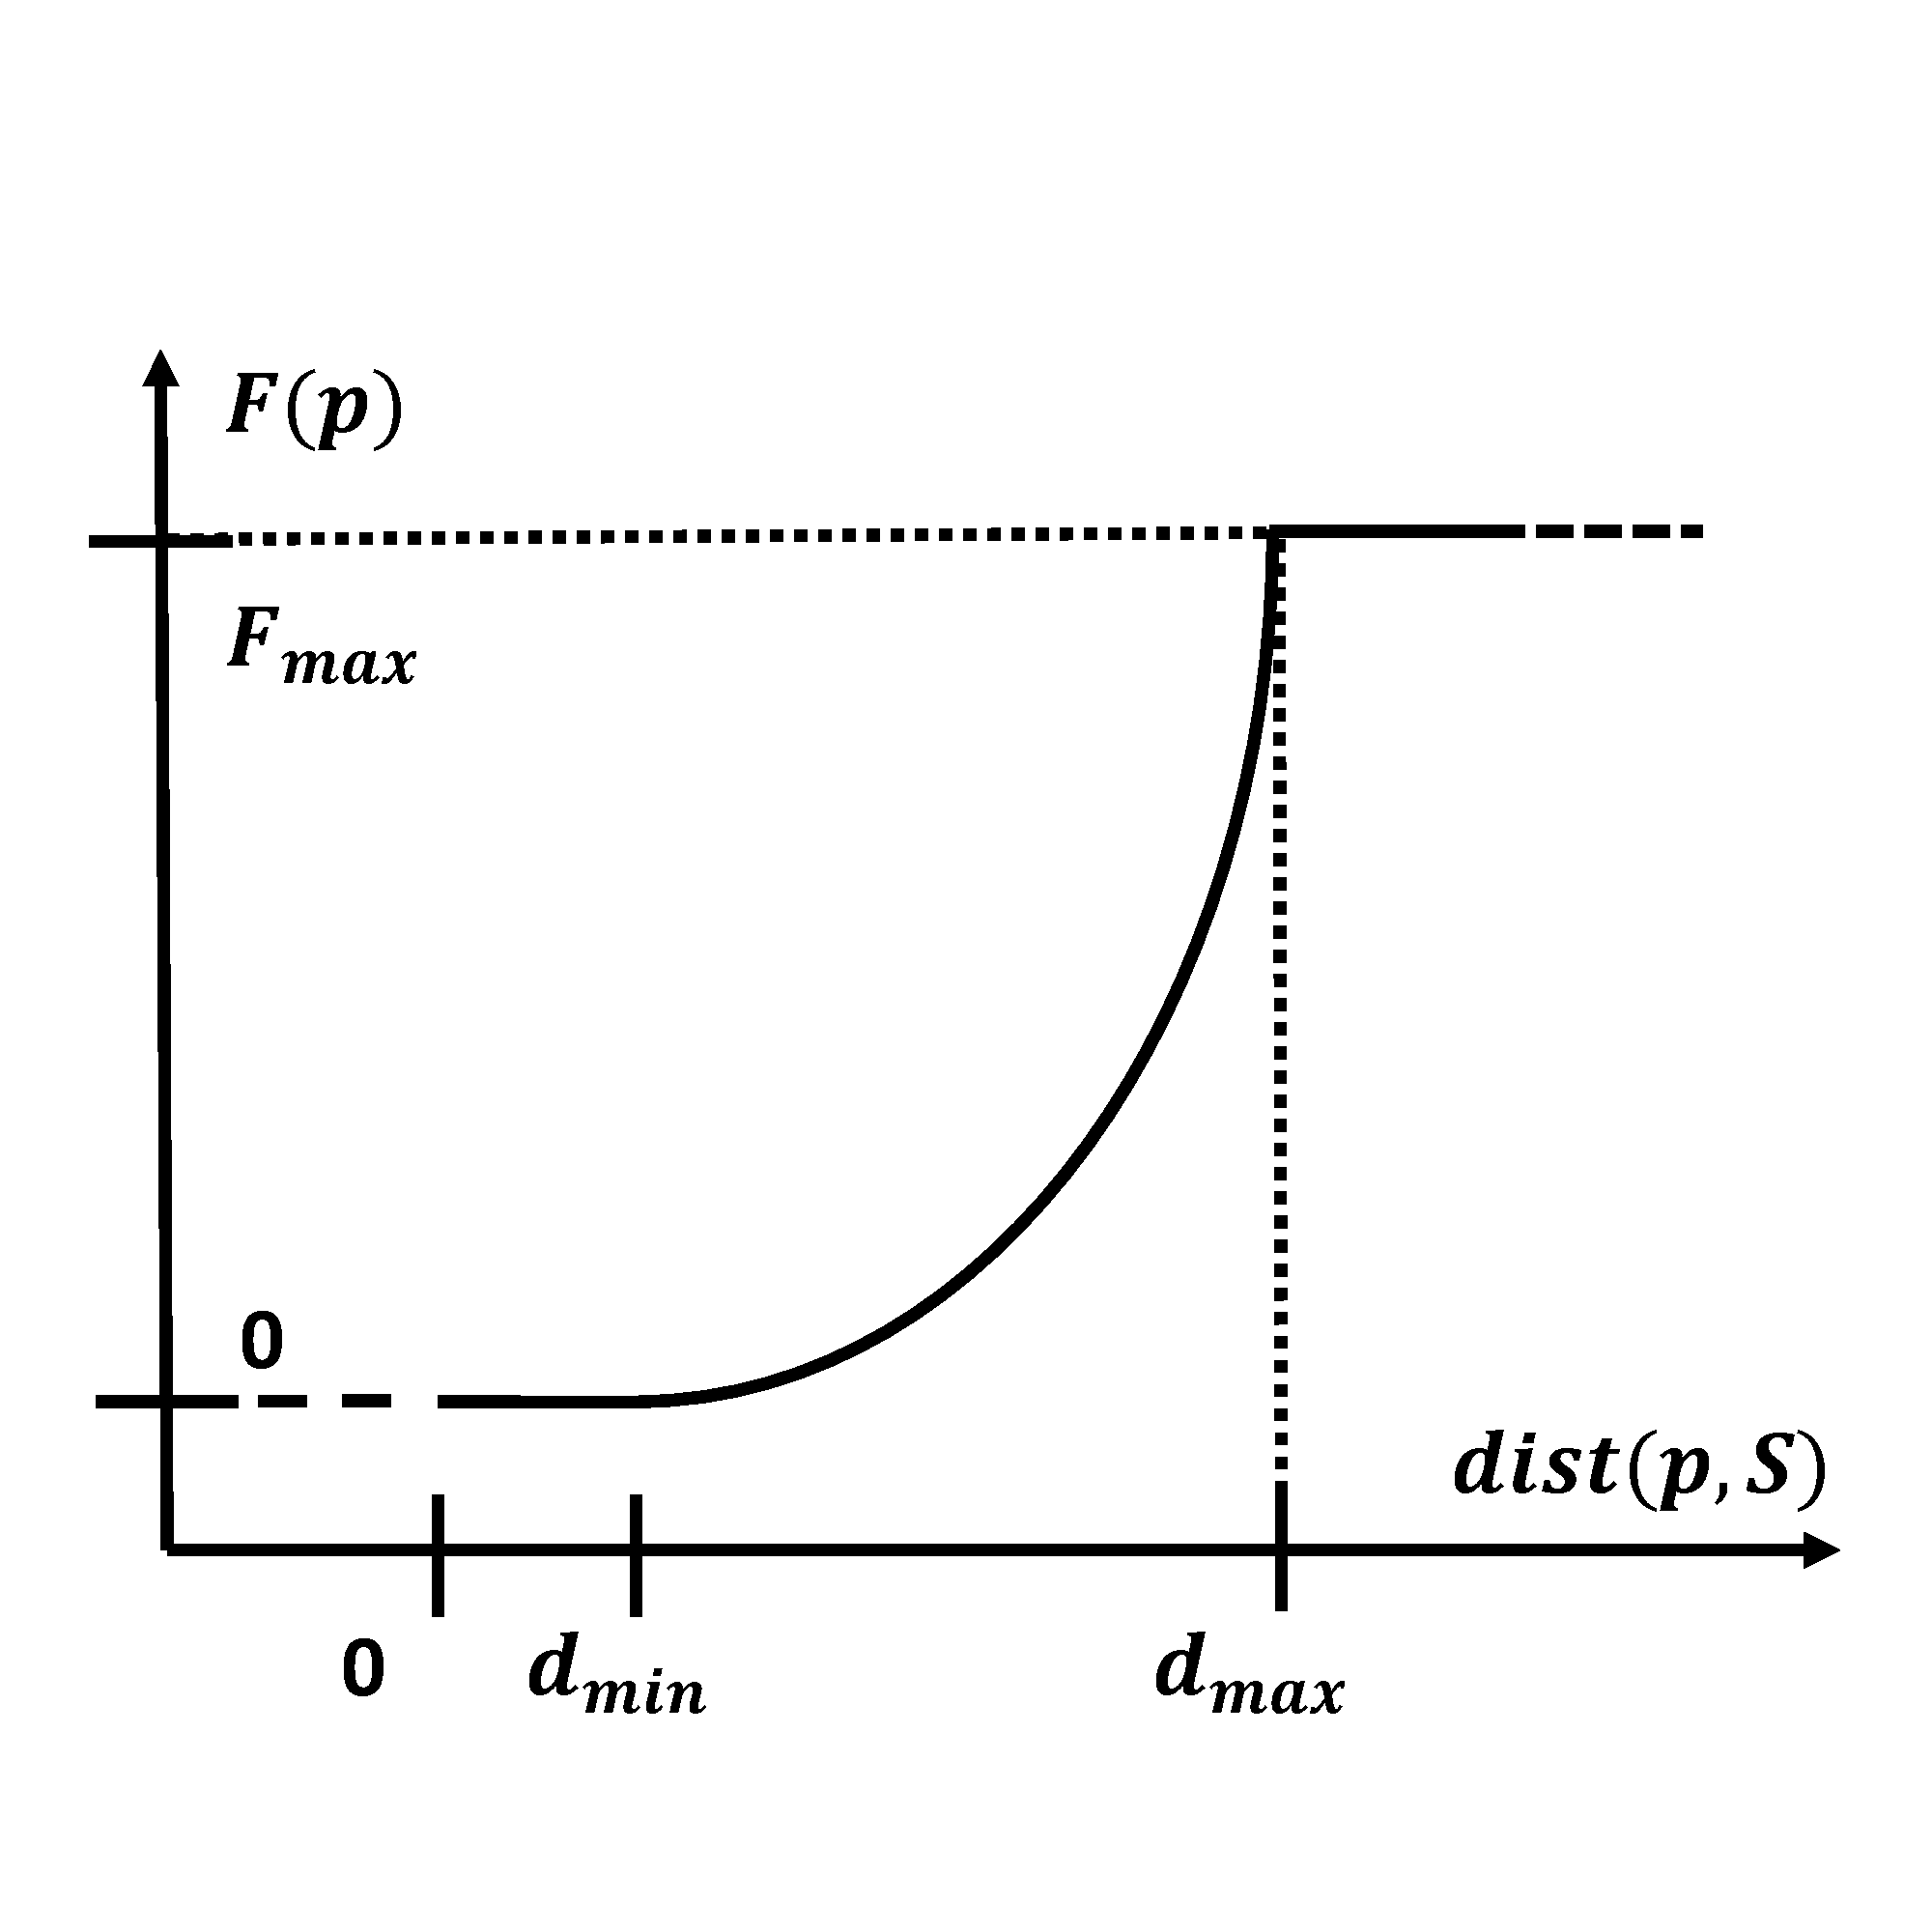
\includegraphics[width=1.0\linewidth]{figs/forbidden.pdf}
% \caption{Forbidden Zone}
% \label{fig:forbidden}
% \end{figure}

\subsubsection{Regularity}
In order to obtain a regular Zometool structure for simple assembling, we intend to regularize the angles between struts to be exact $90^\circ$ and penalize angle that is too small or too big (see \figname~\ref{fig:Regularity}).
% If the rods are too closer to each other, it is hard to construct them. 
% We hope the rods become discrete and the structure have suitable angle for construction. Hence, we set the baseline angle to $90^\circ$. This term will make our structure more regular.
\begin{align}
E_{\text{reg}}(\mathcal{Z}) = \frac{1}{|\mathcal{N}_i|} \sum_{p_j\in\mathcal{N}_i} (\text{min}(\theta_{ij})-\frac{\pi}{2}),
\end{align}

\begin{figure}[ht]
\centering
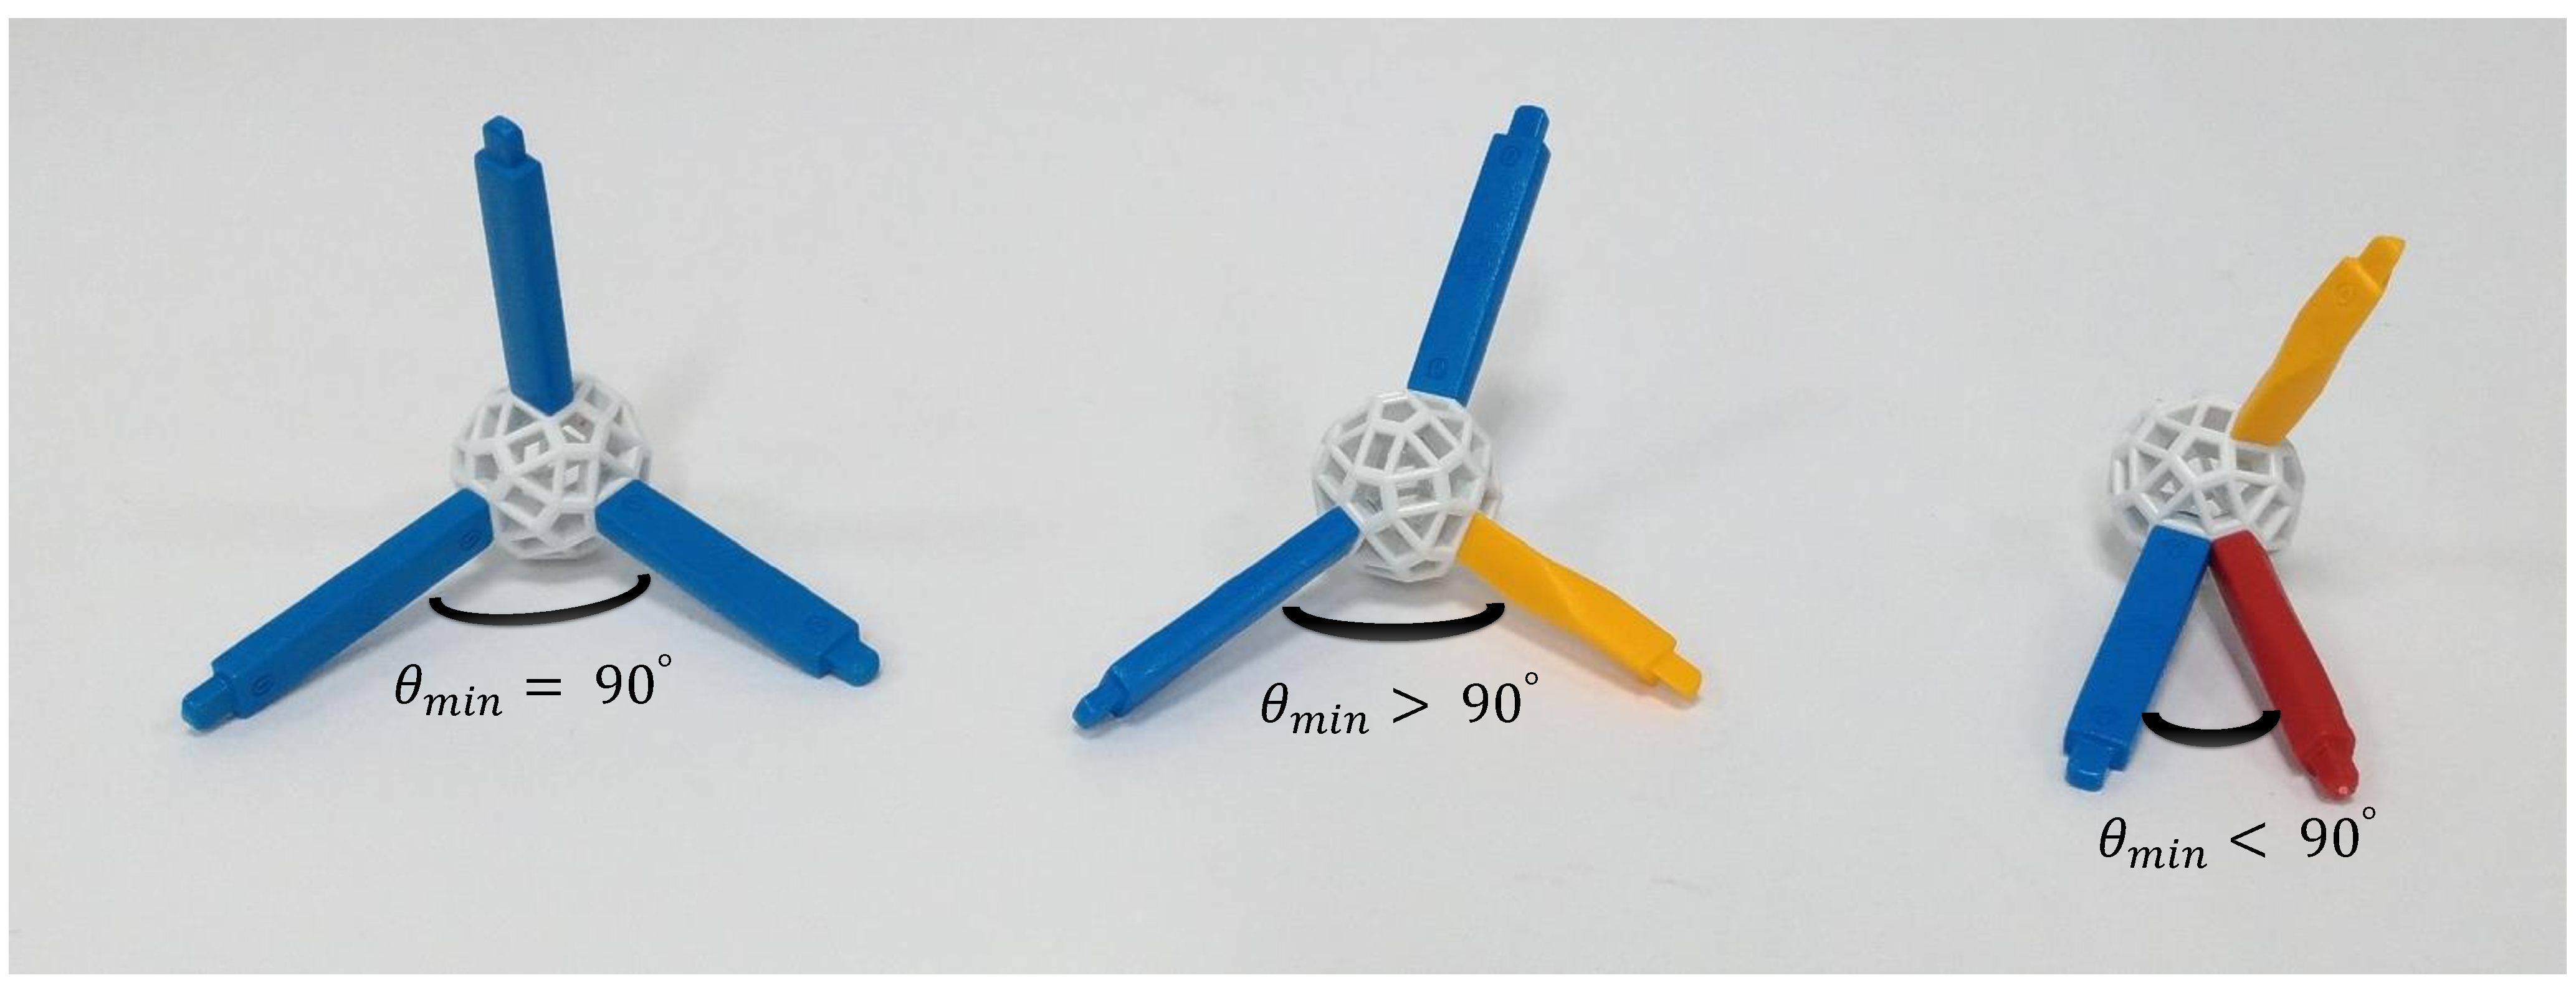
\includegraphics[width=1.0\linewidth]{figs/Regularity.pdf} 
\caption{\textbf{Regularity.} We penalize the configuration with minimum angle between struts smaller or greater than $90^\circ$.}
\label{fig:Regularity}
\end{figure}

\subsubsection{Valence}
We regularize the optimized Zometool structure to have a good valence for simple structure (see \figname~\ref{fig:Valence}). 
In order to maximize each Zome-ball's utility and minimize the complexity, we have to set a baseline number of rods as a constrain.
We set the target valence as $6$ from the initial cube structure.
\begin{align}
E_{\text{val}}(\mathcal{Z}) = \sum_{i=1}^{P} \frac{(V_p-6)^2}{6},
\end{align}
where $V_p$ is the valence of each node.

\begin{figure}[ht]
\centering
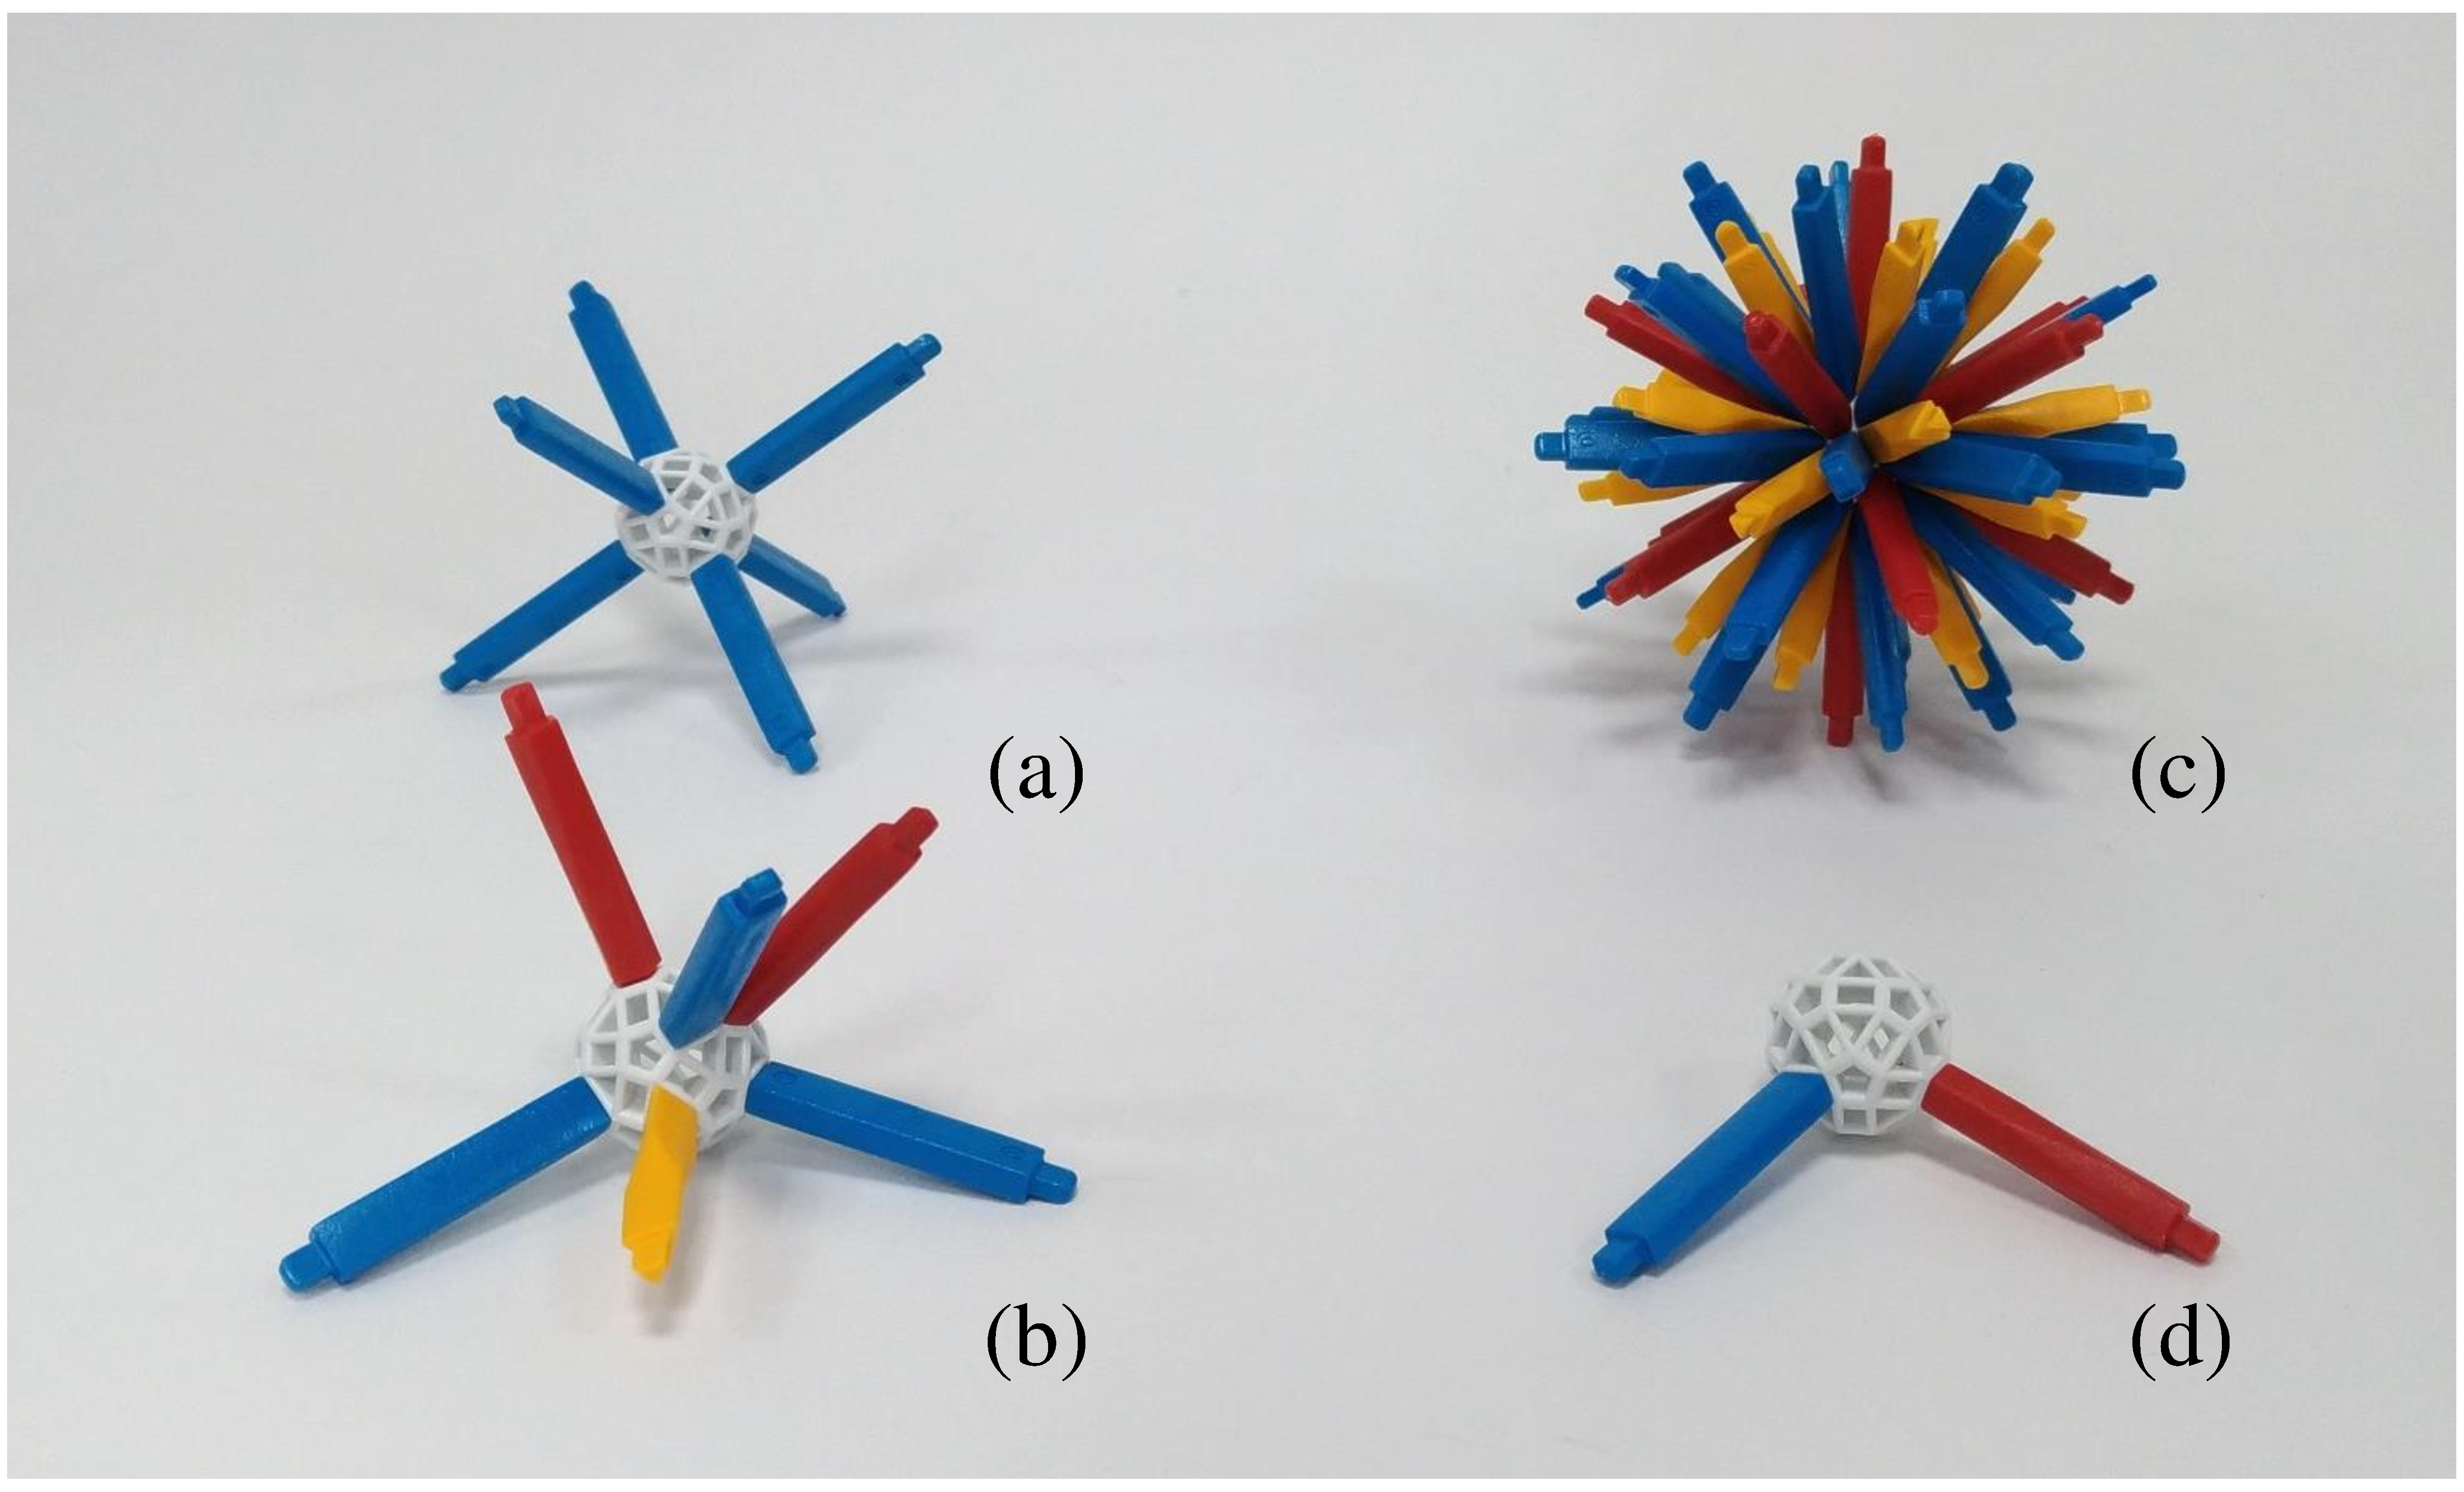
\includegraphics[width=1.0\linewidth]{figs/Valence.pdf} 
\caption{\textbf{Valence.} We encourage the valence of each Zometool node to be 6 (as in configuration (a) and (b)). 
We penalize the valence that is not 6 (configuration (c) and (d)).
}
\label{fig:Valence}
\end{figure}

\subsubsection{Simplicity}
Let $N$ is the total number of both nodes and struts, and $N_\text{target}$ be the target complexity.
The simplicity term is encoded as the quadratic differences from the target complexity:
\begin{align}
E_{\text{sim}}(\mathcal{Z}) = \frac{1}{N_{\text{target}}}(N-N_{\text{target}})^2,
\end{align}
% where $N$ is the total number of both nodes and rods.

\subsection{Exploration Mechanism}
% \ichao{Describe the process of Simulated Anealling}
Searching for the Zometool structure to minimize the energy $E(\mathbf{Z})$ (\eqname~\ref{eq:sa_energy}) is a non trivial optimization problem since $E(\mathbf{Z})$ is non convex and contains global terms. 
Exhaustive search is impractical and thus we adopt a more scalable strategy based on the Metropolis-Hastings algorithm \cite{hastings:1970:monte}.
In a nutshell, this algorithm makes a random exploration of the solution space by iteratively perturbing the current solution with a certain probability depending on the energy variation between the two solutions and a relaxation parameter $T$.
Following, we describe our local perturbation operators and relaxation scheme.
\algoname~\ref{alg:exploration} details the major steps of our optimization algorithm.

\begin{algorithm}[!ht]
\caption{Exploration mechanism}
\label{alg:exploration}
\begin{algorithmic}[1]
\Input{Initialized Zometools $\bar{\mathbf{Z}}$,\\ relaxation parameter $T=T_{init}$}
\Output{Optimized Zometoos $\mathbf{Z}$}
\Procedure{Exploration}{$\mathbf{Z}$}
\Repeat
    \State generate $\mathbf{Z}'$ from $\mathbf{Z}$ with a random local operation.
    \State draw a random value $p \in [0, 1]$ 
    % \State add the collision check here
    \If{$p < \text{exp}(\frac{E(\mathbf{Z})-E(\mathbf{Z}')}{T})$ and CollisionFree($\mathbf{Z}$)} 
        \State update $\mathbf{Z}' \leftarrow \mathbf{Z}$
    \EndIf
    \State Update $T \leftarrow C\times T$ \Comment{Update temperature.}
\Until{$T< T_{end}$}
\EndProcedure
\end{algorithmic}
\end{algorithm}

\subsubsection{Local Perturbation Operation}
During the exploration, we proposed four local perturbation operations (\figname~\ref{fig:local_op}) to construct the Zometool structure by minimizing \eqname~\ref{eq:sa_energy}.
\begin{description}[nosep,itemsep=0pt,leftmargin=0pt]
\item[Split] This operator insert a new node and  two rods to split the original rod.
\item[Merge] This operator insert a new rod to merge two disconnected nodes (two nodes can travel by two edges). 
\item[Bridge] This operator insert a new rod to merge two disconnected nodes (two nodes can't travel by two edges).
\item[Kill] This operator delete a node and two rods.
\end{description}

\begin{figure}[ht]
\centering
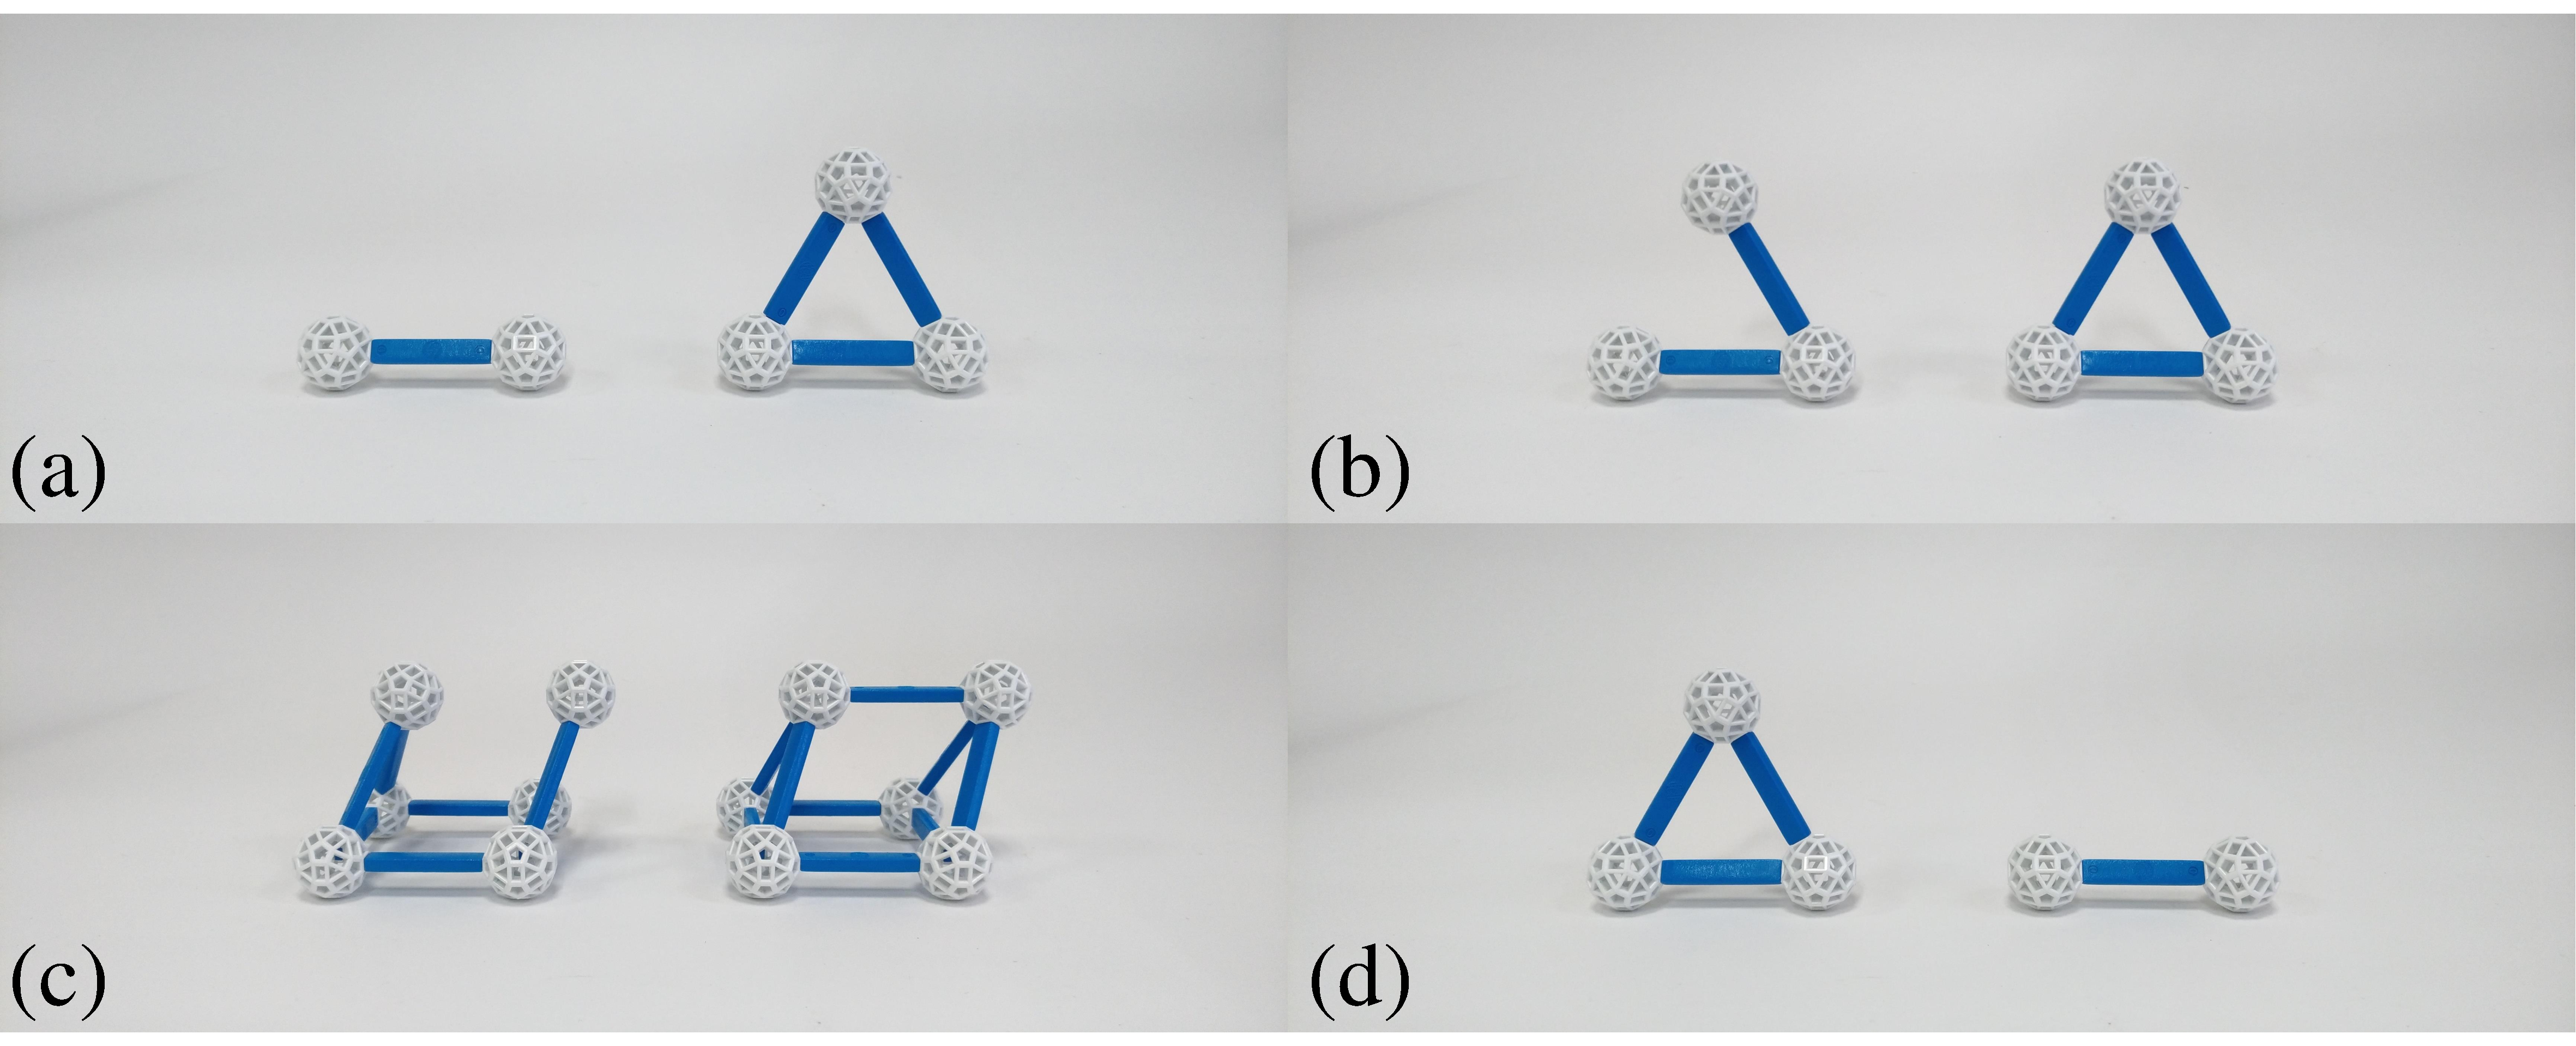
\includegraphics[width=1.0\linewidth]{figs/local_opt.pdf} 
% comment out first for faster compile
% 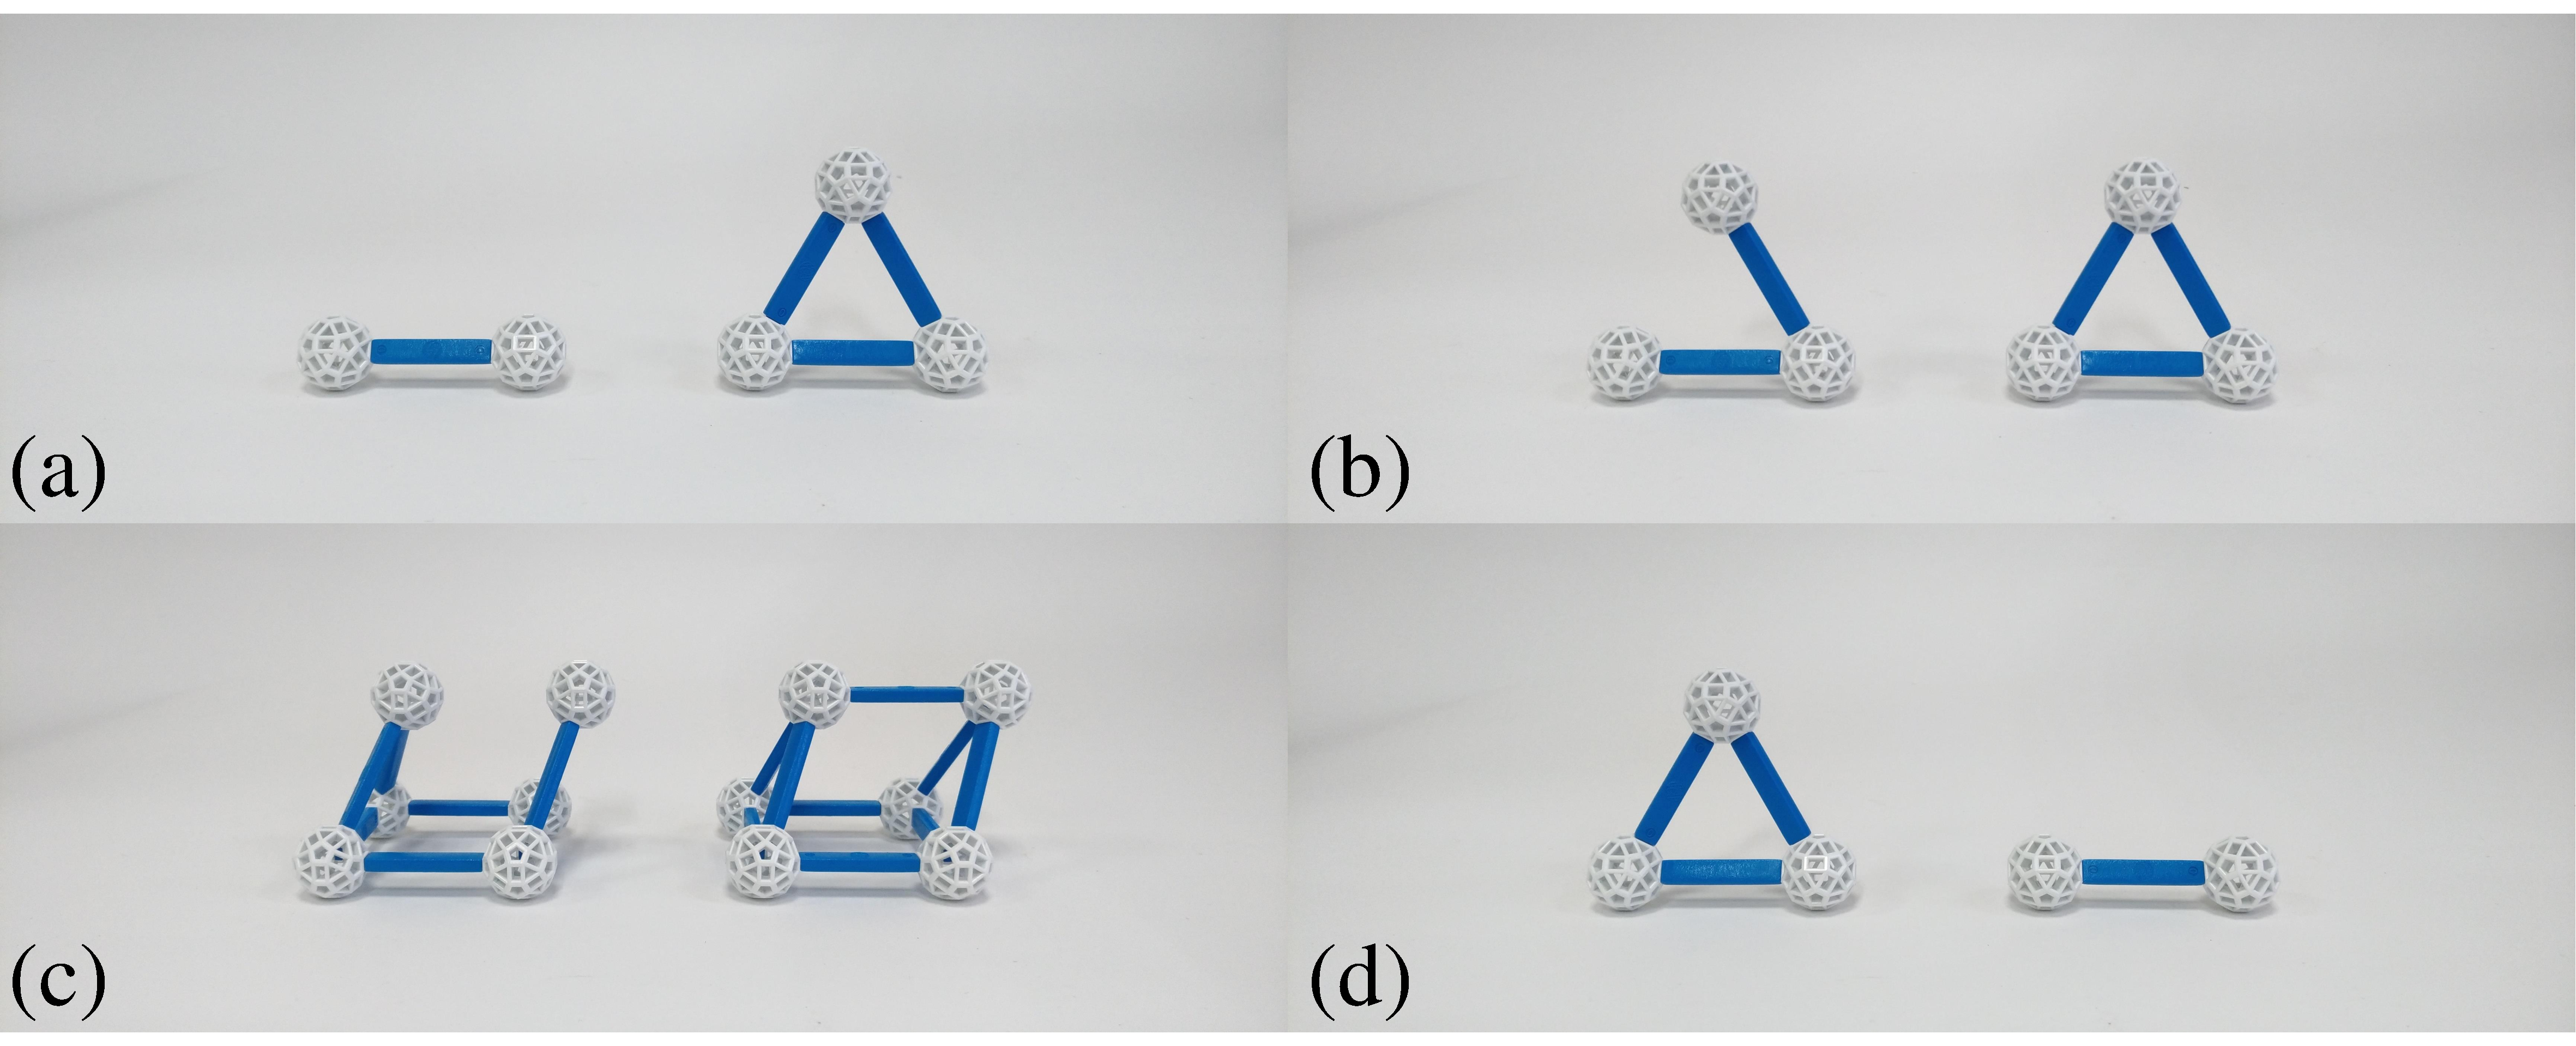
\includegraphics[width=\linewidth]{figs/local_opt.pdf} 
\caption{We use four local operations during structure perturbation. (a) Split, (b) Merge, (c) Bridge, and (d) Kill.}
\label{fig:local_op}
\end{figure}

\paragraph{Operation validity}
The operation will make the structure have some difference from previous round. However, not every round is valid. Our method of judgement which is collision detect is very simple. If the rods or Zome-ball get too close, the collision will happen and the structure will not be assembled. So this procedure will check whether the distance of Zome-ball to Zome-ball, rods to Zome-ball and rods to rods are too close.

\subsubsection{Cooling schedule}
% \ichao{Check what cooling schedule we used..}\\
The relaxation parameter $T$, referred as temperature, controls both the speed and the quality of exploration.
Start from initial temperature $T_{init}$, we decrease the temperature close to zero as iteration tends to infinity.
The decreasing process is referred as cooling, and different cooling schedules are exists for experiment.
Although the global minimum convergence is guaranteed using logarithmic cooling schedule~\cite{Salamon:2002:SA}, we rely on geometric cooling schedule~\cite{Henderson:2003:SA}. 
In our experiment, we set the initial temperature $T_\text{init} = 1$, and the decrease rate $C=0.99$ after every $100$ iterations.